\casoduso{UC1}{Caso d'uso generale} 
\begin{figure}[H] 
\centering 
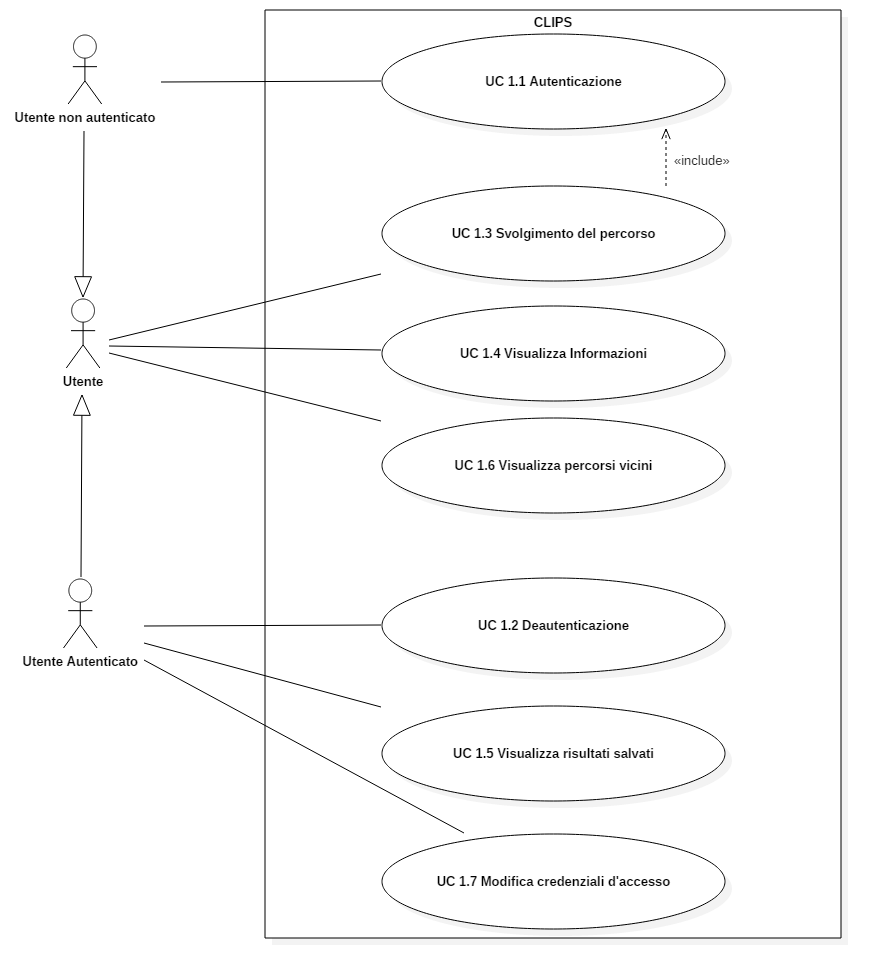
\includegraphics[scale=0.3]{img/UC_1.png} 
\caption{Caso d'uso UC 1} 
 \end{figure} 
\desc{Utente utilizza l'App}\\\\ 
\pre{l'utente ha l'app installata nel dispositivo}\\\\ 
\post{il sistema ha erogato le funzionalità richieste dall'utente}\\\\ 
\scen{l'utente può registrarsi,
l'utente può autenticarsi,
l'utente può deautenticarsi,
l'utente può giocare,
l'utente può ricevere informazioni sull'App,
l'utente registrato può vedere i propri risultati salvati,
l'utente può visualizzare i percorsi vicini.}\\\\ 
\att{Utente}

\casoduso{UC1.1}{Autenticazione} 
\begin{figure}[H] 
\centering 
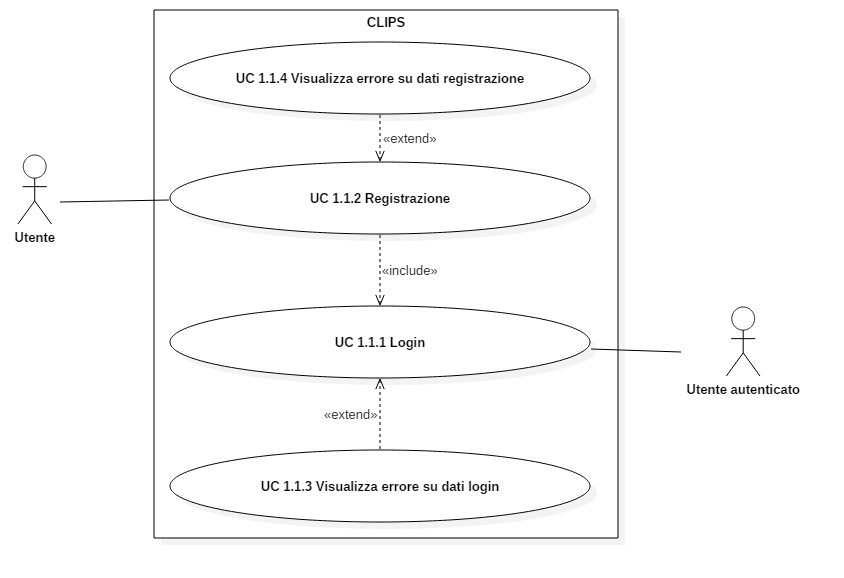
\includegraphics[scale=0.5]{img/UC_1_1.png} 
\caption{Caso d'uso UC 1.1} 
 \end{figure} 
\desc{l'utente può autenticarsi inserendo le proprie credenziali}\\\\ 
\pre{l'utente non è già autenticato}\\\\ 
\post{l'utente è autenticato}\\\\ 
\scen{\UC{1.1.1} l'utente esegue il login se è già registrato,
\UC{1.1.2} l'utente si registra e poi esegue il login (\UC{1.1.1}) se non è registrato.}\\\\ 
\att{Utente non autenticato}

\casoduso{UC1.1.1}{Login} 
\begin{figure}[H] 
\centering 
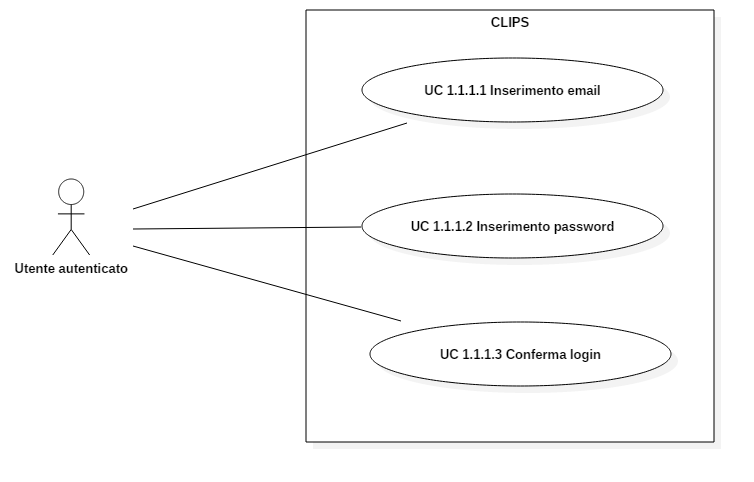
\includegraphics[scale=0.5]{img/UC_1_1_1.png} 
\caption{Caso d'uso UC 1.1.1} 
 \end{figure} 
\desc{l'utente fa il login con le proprie credenziali.

ESTENSIONE:
\UC{UC1.1.3}: l'associazione email/password non esiste nel database.}\\\\ 
\pre{l'utente è registrato presso il database}\\\\ 
\post{l'utente è autenticato}\\\\ 
\scen{\begin{itemize}
\item \UC{UC1.1.1.1} l'utente inserisce l'email,
\item \UC{UC1.1.1.2} l'utente inserisce la password,
\item \UC{UC1.1.1.3} l'utente conferma di voler eseguire il login,
\item ESTENSIONE: se i dati inseriti non sono corretti l'esecuzione prosegue con \UC{UC1.1.3},
\item altrimenti l'utente viene autenticato (\UC{UC1.1.1.4})
\end{itemize}.}\\\\ 
\att{Utente non autenticato}

\casoduso{UC1.1.1.1}{Inserimento email} 
\desc{l'utente inserisce l'indirizzo email con cui si è registrato in precedenza}\\\\ 
\pre{la connessione ad internet è attiva e l'App fornisce la pagina di login}\\\\ 
\post{l'utente ha inserito la mail}\\\\ 
\att{Utente non autenticato}

\casoduso{UC1.1.1.2}{Inserimento password} 
\desc{l'utente inserisce la password con cui si è registrato in precedenza}\\\\ 
\pre{la connessione ad internet è attiva e l'App fornisce la pagina di login}\\\\ 
\post{l'utente ha inserito la password}\\\\ 
\att{Utente non autenticato}

\casoduso{UC1.1.1.3}{Conferma Login} 
\desc{l'utente conferma di voler eseguire il login}\\\\ 
\pre{la connessione ad internet è attiva e l'App fornisce la pagina di login}\\\\ 
\post{l'utente chiede al sistema di essere autenticato}\\\\ 
\scen{Se i dati che vengono confermati sono corretti l'utente viene autenticato (eseguendo \UC{UC1.1.1.4}); altrimenti il sistema informa l'utente della scorrettezza dei dati inseriti tramite l'estensione (\UC{UC1.1.3}).

ESTENSIONE:
\UC{UC1.1.3}}\\\\ 
\att{Utente non autenticato}

\casoduso{UC1.1.1.4}{L'utente viene autenticato} 
\desc{se le informazioni inserite in precedenza sono corrette (in particolare se l'associazione email/password esiste nel sistema) l'utente viene autenticato}\\\\ 
\pre{l'email e la password inserite sono valide}\\\\ 
\post{l'utente è autenticato nel sistema}\\\\ 
\att{Utente non autenticato}

\casoduso{UC1.1.2}{Registrazione} 
\begin{figure}[H] 
\centering 
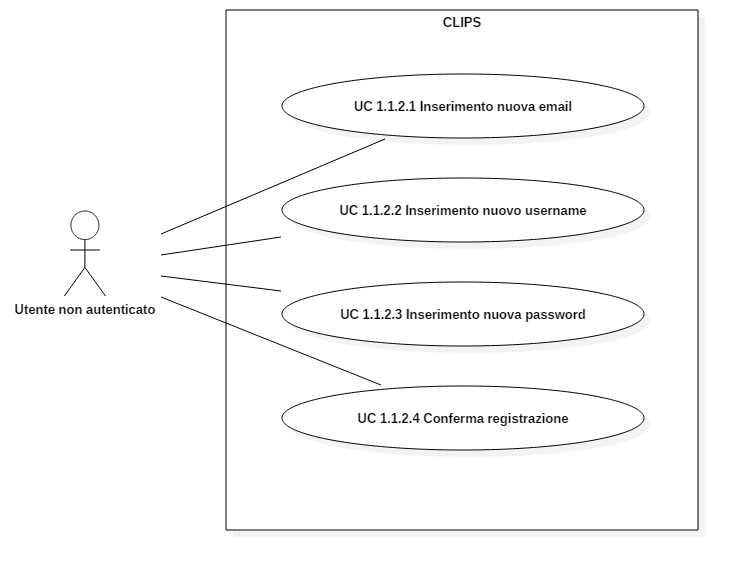
\includegraphics[scale=0.5]{img/UC_1_1_2.png} 
\caption{Caso d'uso UC 1.1.2} 
 \end{figure} 
\desc{l'utente si registra nel database inserendo un'email valida e una password sufficientemente sicura.

INCLUSIONE:
\UC{UC1.1.1}

ESTENSIONE:
l'email non è valida,
l'username è già in uso,
la password non è sufficientemente sicura}\\\\ 
\pre{l'utente non è registrato}\\\\ 
\post{l'utente è registrato nel database}\\\\ 
\scen{l'utente inserisce un indirizzo email valido,
l'utente inserisce un username univoco,
l'utente inserisce una password sufficientemente sicura.}\\\\ 
\att{Utente non autenticato}

\casoduso{UC1.1.2.1}{Inserimento nuova email} 
\desc{l'utente inserisce l'indirizzo email con cui desidera registrarsi}\\\\ 
\pre{la connessione ad internet è attiva e l'App fornisce la pagina di registrazione}\\\\ 
\post{l'utente ha inserito la email}\\\\ 
\att{Utente non autenticato}

\casoduso{UC1.1.2.2}{Inserimento nuovo username} 
\desc{l'utente inserisce l'username con cui desidera registrarsi}\\\\ 
\pre{la connessione ad internet è attiva e l'App fornisce la pagina di registrazione}\\\\ 
\post{l'utente ha inserito l'username}\\\\ 
\att{Utente non autenticato}

\casoduso{UC1.1.2.3}{Inserimento nuova password} 
\desc{l'utente inserisce la password con cui desidera registrarsi}\\\\ 
\pre{la connessione ad internet è attiva e l'App fornisce la pagina di registrazione}\\\\ 
\post{l'utente ha inserito la password}\\\\ 
\att{Utente non autenticato}

\casoduso{UC1.1.2.4}{Conferma Registrazione} 
\desc{l'utente conferma di voler eseguire la registrazione}\\\\ 
\pre{la connessione ad internet è attiva e l'App fornisce la pagina di registrazione}\\\\ 
\post{l'utente chiede al sistema di essere registrato}\\\\ 
\att{Utente non autenticato}

\casoduso{UC1.1.3}{Visualizza errore su dati Login} 
\desc{l'associazione email/password non esiste nel nel database, quindi viene notificato all'utente che l'email o la password inserite sono errate}\\\\ 
\pre{l'utente inserisce dei dati di login errati}\\\\ 
\post{l'utente visualizza l'errore sul login e può inserire nuovamente le credenziali.}\\\\ 
\scen{\UC{UC1.1.3.1} l'utente visualizza l'informazione che i dati inseriti sono errati,
\UC{UC1.1.3.2} l'utente può resettare la propria password}\\\\ 
\att{Utente non autenticato}

\casoduso{UC1.1.3.1}{Visualizza info dati login errati} 
\desc{l'utente visualizza un breve testo che lo informa della scorrettezza dei dati inseriti}\\\\ 
\pre{l'utente inserisce una associazione email/password inesistente}\\\\ 
\post{l'utente è informato della scorrettezza dei dati inseriti}\\\\ 
\att{Utente non autenticato}

\casoduso{UC1.1.3.2}{Resetta la password} 
\desc{l'utente non autenticato che abbia smarrito la password può resettare la password: una password casuale valida viene sostituita a quella correntemente associata all'indirizzo email e viene inviata allo stesso indirizzo (insieme ad un invito ad aggiornarla al più presto).}\\\\ 
\pre{l'utente non è autenticato e desidera effettuare il reset della password}\\\\ 
\post{l'utente trova la nuova password nella propria casella di posta}\\\\ 
\att{Utente non autenticato}

\casoduso{UC1.1.4}{Visualizza errore su dati registrazione} 
\desc{l'utente compie uno dei seguenti errore e viene notificato per ciò:
- l'email inserita non è valida,
- l'username inserito non è disponibile
- la password non è sufficientemente sicura}\\\\ 
\pre{l'utente inserisce dei dati di registrazione non validi}\\\\ 
\post{l'utente visualizza l'errore sulla registrazione e può correggere i campi errati}\\\\ 
\att{Utente non autenticato}

\casoduso{UC1.2}{Deautenticazione} 
\desc{l'utente autenticato esegue il logout}\\\\ 
\pre{l'utente è autenticato}\\\\ 
\post{l'utente non è più autenticato}\\\\ 
\att{Utente autenticato}

\casoduso{UC1.3}{Svolgimento del Percorso} 
\begin{figure}[H] 
\centering 
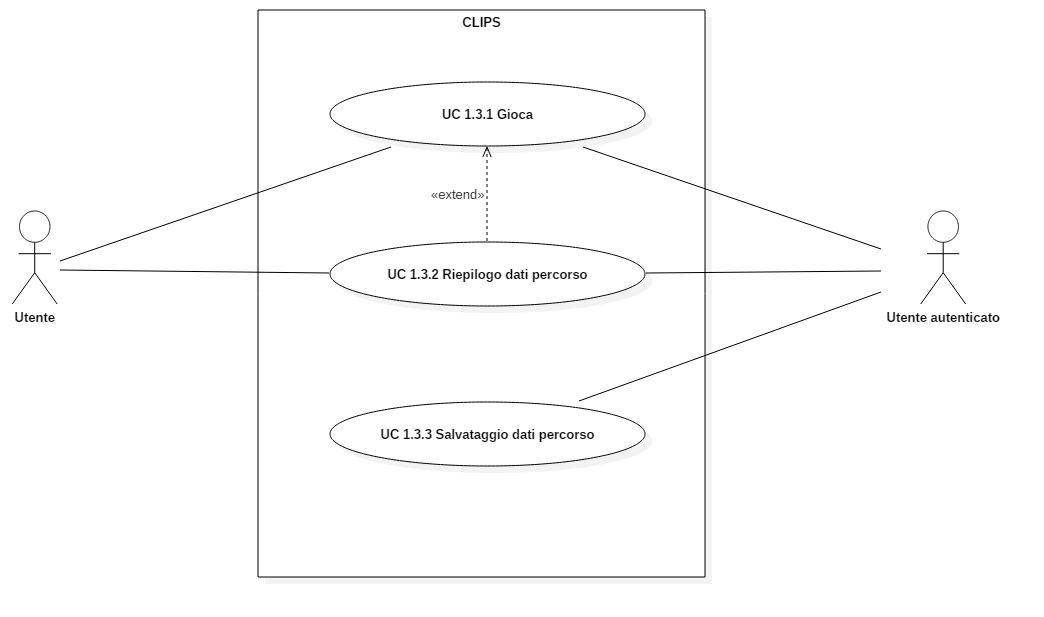
\includegraphics[scale=0.4]{img/UC_1_3.png} 
\caption{Caso d'uso UC 1.3} 
 \end{figure} 
\desc{l'utente svolge un percorso tra quelli disponibili nel luogo in cui si trova.}\\\\ 
\pre{l'utente ha i servizi di localizzazione, Bluetooth e connessione ad internet attivi e si trova in un luogo abilitato.}\\\\ 
\post{l'utente ha completato il percorso selezionato.}\\\\ 
\scen{l'utente effettua i seguenti passi:
\begin{itemize}
\item \UC{1.3.1} l'utente gioca il percorso,
\item \UC{1.3.2} l'utente visualizza i dati del percorso appena concluso,
\end{itemize}
a questo punto gli utenti autenticati hanno la possibilità di registrare i progressi effettuati, quindi viene data l'opportunità agli utenti non autenticati di autenticarsi tramite: \\
INCLUSIONE:
l'utente non autenticato ha l'opportunità di autenticarsi (\UC{1.1}),
a questo punto, gli utenti che ora sono autenticati possono procedere con:
\begin{itemize}
\item \UC{1.3.3} l'utente autenticato salva i risultati.
\end{itemize}.}\\\\ 
\att{Utente}

\casoduso{UC1.3.1}{Gioca} 
\begin{figure}[H] 
\centering 
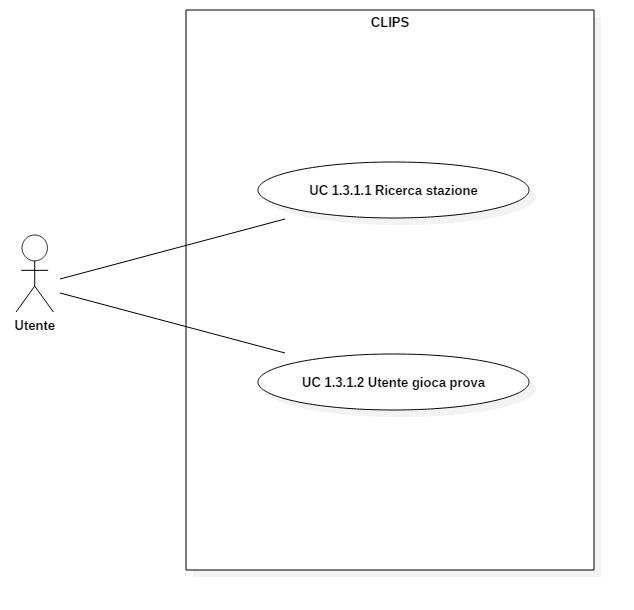
\includegraphics[scale=0.5]{img/UC_1_3_1.png} 
\caption{Caso d'uso UC 1.3.1} 
 \end{figure} 
\desc{l'utente si trova in un luogo abilitato, scarica un percorso e lo conclude.}\\\\ 
\pre{l'utente ha scelto un percorso.}\\\\ 
\post{l'utente completa tutte le prove.}\\\\ 
\scen{\UC{UC1.3.1.1} l'utente raggiunge la stazione,
\UC{UC1.3.1.2} l'utente svolge la prova della stazione in cui si trova,
\UC{UC1.3.1.3} l'utente viene invitato a cercare la prova seguente.

ESTENSIONE:
 - Se la prova conclusa è l'ultima l'utente visualizza il riepilogo \UC{UC1.3.2}}\\\\ 
\att{Utente}

\casoduso{UC1.3.1.1}{Ricerca stazione} 
\desc{l'utente è alla ricerca della stazione in cui recarsi per la prossima (o la prima) prova}\\\\ 
\pre{l'utente non sta svolgendo alcuna prova e non ha concluso il percorso}\\\\ 
\post{l'utente è presso la stazione in cui svolgere la prossima prova}\\\\ 
\att{Utente}

\casoduso{UC1.3.1.2}{Utente gioca prova} 
\begin{figure}[H] 
\centering 
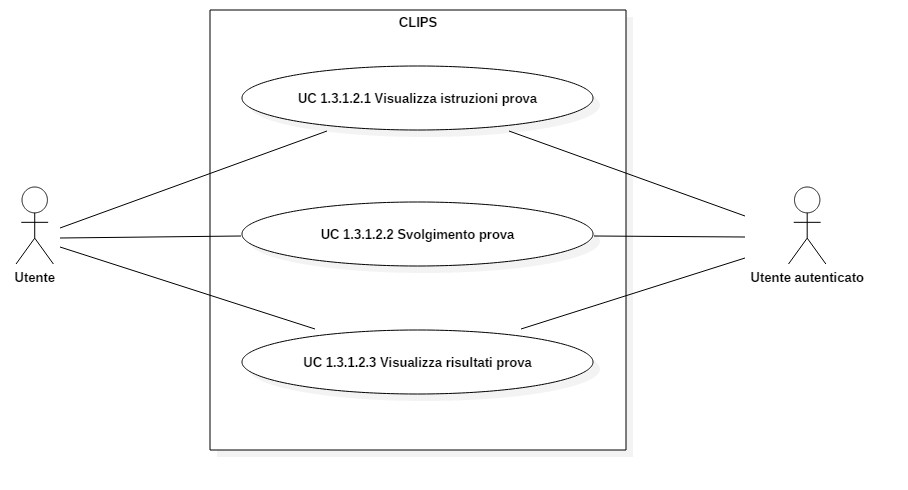
\includegraphics[scale=0.5]{img/UC_1_3_1_2.png} 
\caption{Caso d'uso UC 1.3.1.2} 
 \end{figure} 
\desc{l'utente affronta la prova della stazione in cui si trova}\\\\ 
\pre{l'utente si trova nella sua prossima stazione}\\\\ 
\post{l'utente ha completato la prova}\\\\ 
\scen{- \UC{UC1.3.1.2.1} l'utente visualizza una descrizione della prova
- \UC{UC1.3.1.2.2} l'utente gioca la prova
- \UC{UC1.3.1.2.3} l'utente ottiene un punteggio sulla prova}\\\\ 
\att{Utente}

\casoduso{UC1.3.1.2.1}{Visualizza istruzioni prova} 
\desc{l'utente visualizza le informazioni che l'utente deve sapere in preparazione alla prova, solitamente le istruzioni; a questo punto il tempo per la prova non scorre ancora.}\\\\ 
\pre{l'utente è in procinto di iniziare la prova}\\\\ 
\post{l'utente è informato di come procedere per la prova}\\\\ 
\att{Utente}

\casoduso{UC1.3.1.2.2}{Svolgimento prova} 
\desc{l'utente svolge la prova}\\\\ 
\pre{l'utente ha visualizzato le informazioni necessarie allo svolgimento della prova}\\\\ 
\post{l'utente ha concluso la prova con successo}\\\\ 
\scen{Viene conclusa la prova prevista per la stazione.}\\\\ 
\att{Utente}

\casoduso{UC1.3.1.2.3}{Visualizza risultati prova} 
\desc{l'utente viene informato circa i risultati ottenuti durante la prova appena conclusa}\\\\ 
\pre{l'utente ha appena concluso una prova}\\\\ 
\post{l'utente ottiene i risultati circa la prova appena conclusa}\\\\ 
\att{Utente}

\casoduso{UC1.3.2}{Riepilogo dati 
percorso} 
\begin{figure}[H] 
\centering 
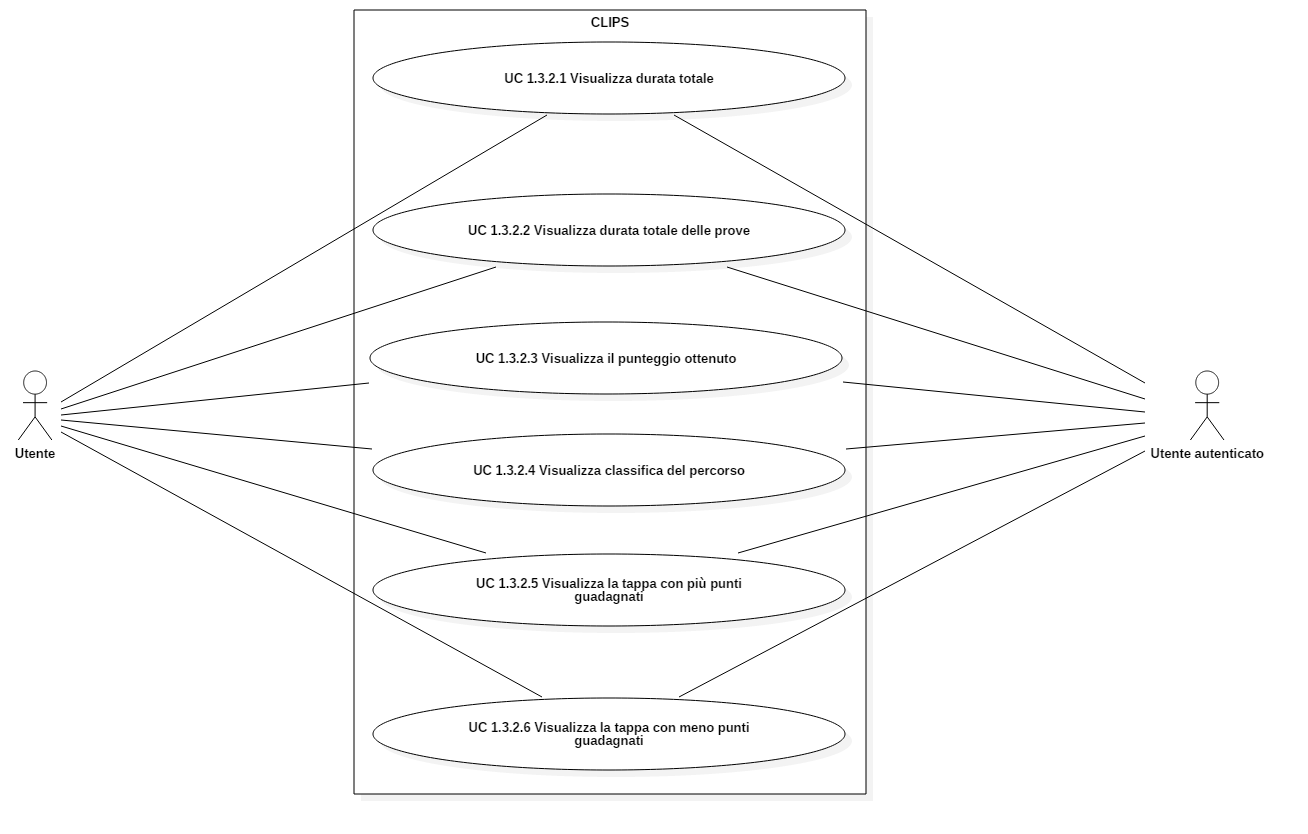
\includegraphics[scale=0.3]{img/UC_1_3_2.png} 
\caption{Caso d'uso UC 1.3.2} 
 \end{figure} 
\desc{dopo che l'utente termina il percorso, visualizza il riassunto (durata totale, durata totale delle prove, punteggio ottenuto, posizione in classifica).}\\\\ 
\pre{l'utente ha completato il percorso}\\\\ 
\post{l'app presenta il riassunto del percorso}\\\\ 
\scen{l'utente visualizza le seguenti informazioni:
 - \UC{UC1.3.2.1} informazioni generali sulla durata (orario di inizio/fine, durata totale),
 - \UC{UC1.3.2.2} durata delle prove (somma della durata di ciascuna prova),
 - \UC{UC1.3.2.3} punteggio ottenuto ottenuto (somma dei punteggi ottenuti nelle varie prove),
 - \UC{UC1.3.2.4} punteggio medio ottenuto dagli utenti (media dei punteggi ottenuti su quel percorso),
 - \UC{UC1.3.2.5} visualizza la tappa in cui è stato ottenuto il maggior numero di punti,
 - \UC{UC1.3.2.6} visualizza la tappa in cui è stato ottenuto il minor numero di punti.}\\\\ 
\att{Utente}

\casoduso{UC1.3.2.1}{Visualizza durata totale} 
\desc{Visualizza la durata totale del percorso (il tempo intercorso tra l'orario di inizio e quello di fine).}\\\\ 
\pre{l'utente ha concluso il percorso}\\\\ 
\post{l'app mostra i dettagli sul tempo di inizio, fine e durata.}\\\\ 
\att{Utente}

\casoduso{UC1.3.2.2}{Visualizza durata totale delle prove} 
\desc{Visualizza la durata totale del percorso (la somma dei tempi spesi dall'utente nel compiere le varie prove).}\\\\ 
\pre{l'utente ha concluso il percorso}\\\\ 
\post{l'app mostra i dettagli sulla durata delle prove.}\\\\ 
\att{Utente}

\casoduso{UC1.3.2.3}{Visualizza il punteggio ottenuto} 
\desc{Visualizza il punteggio ottenuto durante il percorso (la somma dei punteggi ottenuti nelle varie prove).}\\\\ 
\pre{l'utente ha concluso il percorso}\\\\ 
\post{l'app mostra il punteggio ottenuto.}\\\\ 
\att{Utente}

\casoduso{UC1.3.2.4}{Visualizza classifica del percorso} 
\desc{Visualizza alcune informazioni circa le prime posizioni in classifica, quelle antecedenti e quelle seguenti l'utente nel percorso appena concluso (si veda \Req{R0F3.2.4} e figli.}\\\\ 
\pre{l'utente ha concluso il percorso}\\\\ 
\post{l'app mostra la posizione in classifica assoluta ottenuta per quel percorso}\\\\ 
\att{Utente}

\casoduso{UC1.3.2.5}{Visualizza la tappa con più punti guadagnati} 
\desc{Visualizza la tappa del percorso appena concluso in cui l'utente ha accumulato il maggior numero di punti.}\\\\ 
\pre{l'utente ha concluso il percorso}\\\\ 
\post{l'app mostra la prova in cui l'utente ha accumulato il maggior numero di punti}\\\\ 
\att{Utente}

\casoduso{UC1.3.2.6}{Visualizza la tappa con meno punti guadagnati} 
\desc{Visualizza la tappa del percorso appena concluso in cui l'utente ha accumulato il minor numero di punti.}\\\\ 
\pre{l'utente ha concluso il percorso}\\\\ 
\post{l'app mostra la prova in cui l'utente ha accumulato il minor numero di punti}\\\\ 
\att{Utente}

\casoduso{UC1.3.3}{Salvataggio dati percorso} 
\desc{l'utente autenticato può salvare i dati relativi al percorso appena conclusosi.}\\\\ 
\pre{si è concluso il percorso, l'utente è autenticato}\\\\ 
\post{i dati del percorso vengono salvati nel database per una futura consultazione}\\\\ 
\att{Utente autenticato}

\casoduso{UC1.4}{Visualizza Informazioni} 
\begin{figure}[H] 
\centering 
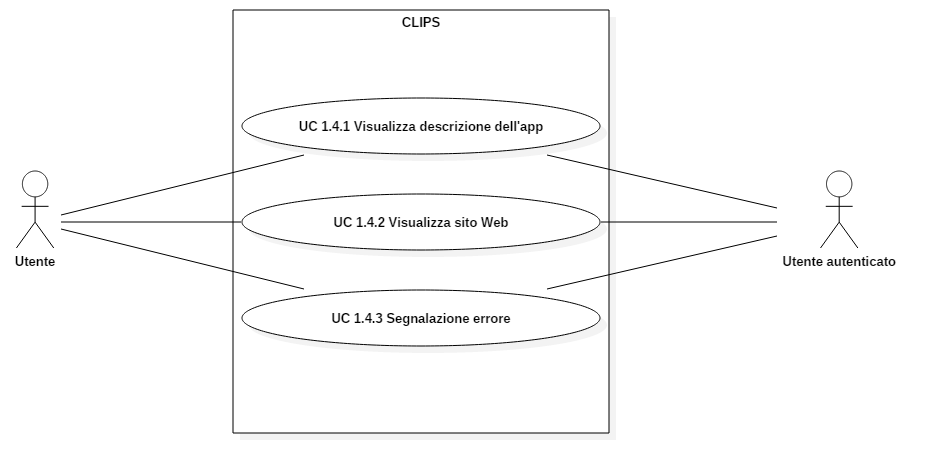
\includegraphics[scale=0.4]{img/UC_1_4.png} 
\caption{Caso d'uso UC 1.4} 
 \end{figure} 
\desc{l'utente visualizza le informazioni relative all'App}\\\\ 
\pre{l'utente ha l'App installata}\\\\ 
\post{l'utente si informa sull'App}\\\\ 
\scen{\UC{UC1.4.1} l'utente visualizza una descrizione delle funzionalità dell'app,
\UC{UC1.4.2} l'utente visita il sito web dell'app,
\UC{UC1.4.3} l'utente contatta il supporto tecnico dell'app.}\\\\ 
\att{Utente}

\casoduso{UC1.4.1}{Visualizza descrizione dell'app} 
\desc{l'utente visualizza una schermata con un testo esplicativo delle funzionalità dell'App}\\\\ 
\pre{l'utente desidera ottenere informazioni sull'App}\\\\ 
\post{l'App mostra all'utente la descrizione delle sue funzionalità}\\\\ 
\att{Utente}

\casoduso{UC1.4.2}{Visualizza sito Web} 
\desc{l'utente desidera visualizzare il sito web relativo all'App per ottenere maggiori informazioni a riguardo}\\\\ 
\pre{l'utente desidera visitare il sito web}\\\\ 
\post{l'app apre nel browser del dispositivo il sito web relativo}\\\\ 
\att{Utente}

\casoduso{UC1.4.3}{Segnalazione errore} 
\desc{L'utente crede che ci sia un errore nel funzionamento dell'app e lo segnala}\\\\ 
\pre{l'utente desidera segnalare un malfunzionamento}\\\\ 
\post{l'app fornisce all'utente la possibilità di inviare un'email al supporto dell'app tramite il client email di default nel dispositivo}\\\\ 
\scen{si apre il client email di default nel dispositivo con il campo destinatario impostato all'indirizzo di supporto dell'app,
l'utente invia una richiesta di supporto.}\\\\ 
\att{Utente}

\casoduso{UC1.5}{Visualizza i Risultati Salvati} 
\begin{figure}[H] 
\centering 
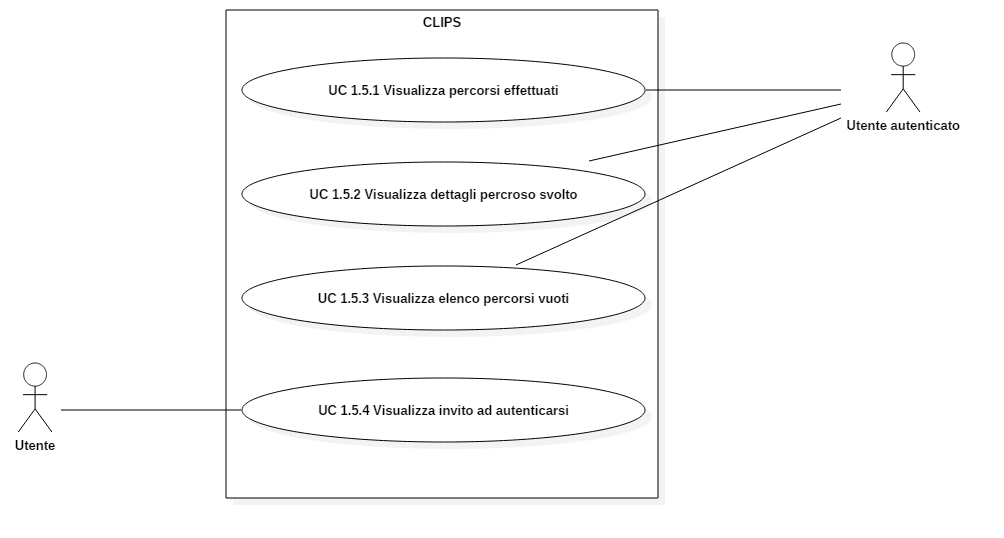
\includegraphics[scale=0.4]{img/UC_1_5.png} 
\caption{Caso d'uso UC 1.5} 
 \end{figure} 
\desc{l'utente autenticato visualizza i risultati salvati in precedenza}\\\\ 
\pre{l'utente desidera visualizzare informazioni circa gli scenari visualizzati}\\\\ 
\post{l'utente visualizza i dati relativi ai percorsi già compiuti (se ce ne sono) o gli viene spiegato perché ciò non è possibile}\\\\ 
\scen{se l'utente non è autenticato:
 - \UC{UC1.5.3} l'utente viene informato della possibilità di salvare i percorsi effettuati se si autentica,
altrimenti, se l'utente non ha percorsi registrati:
 - \UC{UC1.5.2} l'utente viene invitato a compiere un percorso per poi visualizzarne il dettaglio in questa pagina
altrimenti:
 - \UC{UC1.5.1} l'utente visualizza l'elenco dei percorsi svolti,
 - \UC{UC1.5.1.1} l'utente può visualizzare il dettaglio di un percorso salvato.}\\\\ 
\att{Utente}

\casoduso{UC1.5.1}{Visualizza percorsi effettuati} 
\desc{l'utente autenticato visualizza l'elenco dei percorsi effettuati, visualizzando qualche informazione associata (data percorso, punteggio raggiunto, …)}\\\\ 
\pre{l'utente è autenticato e ha già concluso qualche percorso}\\\\ 
\post{l'app mostra all'utente alcune informazioni sui percorsi svolti}\\\\ 
\att{Utente autenticato}

\casoduso{UC1.5.1.1}{Visualizza dettagli percorso svolto} 
\desc{l'utente autenticato desidera visualizzare tutte le informazioni relative ad un percorso effettuato (luogo, data, ora di inizio, ora di fine, tempo totale speso nelle prove, punteggio finale, …)}\\\\ 
\pre{l'utente è autenticato, ha qualche percorso salvato nell'account e ha selezionato un percorso da visualizzare in dettaglio}\\\\ 
\post{l'app mostra il dettaglio del percorso selezionato}\\\\ 
\att{Utente autenticato}

\casoduso{UC1.5.2}{Visualizza elenco percorsi vuoto} 
\desc{se l'utente è autenticato ma non ha mai svolto alcun percorso, l'app mostrerà una breve spiegazione del perché non si vede alcun percorso (nessuno è stato svolto finora) e invita l'utente a completarne uno.}\\\\ 
\pre{l'utente è autenticato e non ha alcun percorso registrato nel suo account}\\\\ 
\post{l'app presenta all'utente un testo di chiarificazione della pagina}\\\\ 
\att{Utente autenticato}

\casoduso{UC1.5.3}{Visualizza invito ad autenticarsi} 
\desc{l'app mostra all'utente non autenticato una schermata in cui spiega che se l'utente si autentica potrà salvare i risultati dei percorsi e, in questa schermata, visualizzarli.}\\\\ 
\pre{l'utente non è autenticato}\\\\ 
\post{l'app informa l'utente della funzionalità di salvataggio dei percorsi disponibile per i soli utenti autenticati}\\\\ 
\att{Utente non autenticato}

\casoduso{UC1.6}{Visualizza percorsi vicini} 
\begin{figure}[H] 
\centering 
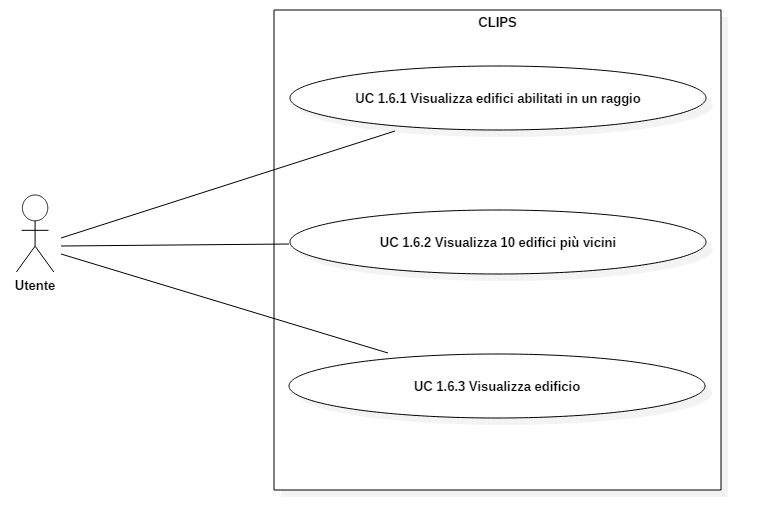
\includegraphics[scale=0.4]{img/UC_1_6.png} 
\caption{Caso d'uso UC 1.6} 
 \end{figure} 
\desc{l'utente visualizza i percorsi nelle vicinanze (o i più vicini)}\\\\ 
\pre{l'utente ha i servizi di localizzazione attivi, l'utente ha la connessione ad internet attiva.}\\\\ 
\post{l'utente visualizza i percorsi disponibili nelle vicinanze.}\\\\ 
\scen{\UC{1.6.1} l'utente visualizza gli edifici abilitati entro un certo raggio,
\UC{1.6.2} l'utente visualizza i 10 edifici più vicini.}\\\\ 
\att{Utente}

\casoduso{UC1.6.1}{Visualizza edifici abilitati in un raggio} 
\begin{figure}[H] 
\centering 
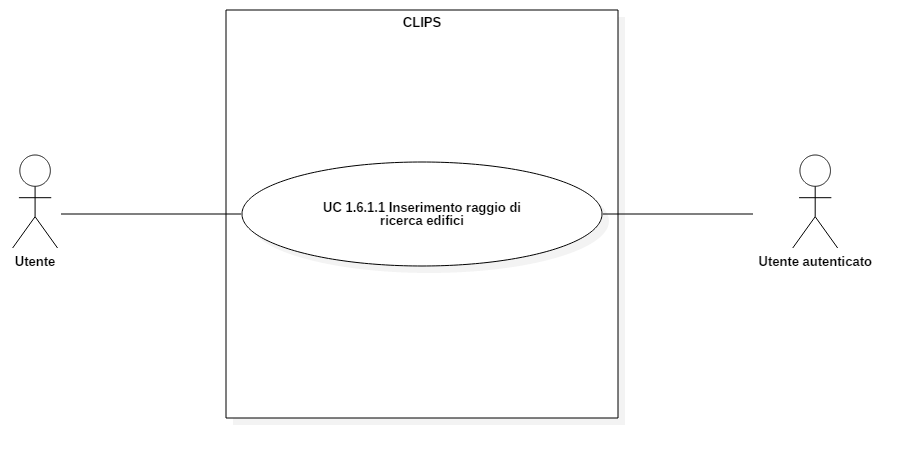
\includegraphics[scale=0.5]{img/UC_1_6_1.png} 
\caption{Caso d'uso UC 1.6.1} 
 \end{figure} 
\desc{l'utente vuole sapere quali sono gli edifici abilitati (con percorsi) nelle vicinanze ed imposta un raggio per effettuare la ricerca.}\\\\ 
\pre{l'utente ha i servizi di localizzazione attivi, una connessione ad internet ed ha inserito il raggio (in km) entro cui desidera cercare edifici abilitati}\\\\ 
\post{l'app mostra all'utente gli edifici abilitati entro il raggio impostato}\\\\ 
\scen{\UC{UC1.6.1.1} l'utente inserisce un raggio entro cui effettuare la ricerca di edifici abilitati}\\\\ 
\att{Utente}

\casoduso{UC1.6.1.1}{Inserimento raggio di ricerca edifici} 
\desc{l'utente inserisce un raggio (in km) entro il quale ricercare edifici abilitati (con percorsi).}\\\\ 
\pre{l'utente ha inserito i km entro cui effettuare la ricerca degli edifici}\\\\ 
\post{l'app mostra all'utente la lista degli edifici nel raggio scelto}\\\\ 
\att{Utente}

\casoduso{UC1.6.2}{Visualizza 10 edifici più vicini} 
\desc{l'app mostra all'utente quali sono i 10 edifici più vicini}\\\\ 
\pre{l'utente ha i servizi di localizzazione attivi ed è connesso ad internet}\\\\ 
\post{l'app mostra all'utente i 10 edifici più vicini}\\\\ 
\att{Utente}

\casoduso{UC1.6.3}{Visualizza Edificio} 
\begin{figure}[H] 
\centering 
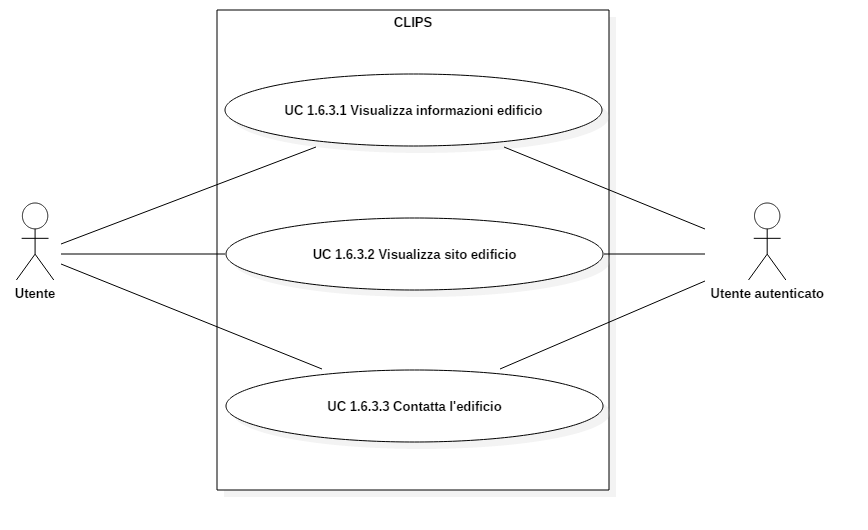
\includegraphics[scale=0.5]{img/UC_1_6_3.png} 
\caption{Caso d'uso UC 1.6.3} 
 \end{figure} 
\desc{l'utente seleziona un edificio dalla lista degli edifici per visualizzarne le informazioni.}\\\\ 
\pre{l'utente è connesso ad internet}\\\\ 
\post{l'app mostra le informazioni riguardanti l'edificio}\\\\ 
\scen{l'utente può ottenere informazioni sull'edificio in diverse maniere:
 - \UC{UC1.6.3.1} attraverso le informazioni 'in-app' sull'edificio,
 - \UC{UC1.6.3.2} accedendo al sito web relativo all'edificio,
 - \UC{UC1.6.3.3} contattando in maniera diretta l'edificio.}\\\\ 
\att{Utente}

\casoduso{UC1.6.3.1}{Visualizza informazioni edificio} 
\desc{l'utente visualizza alcune informazioni sull'edificio}\\\\ 
\pre{l'utente seleziona un edificio}\\\\ 
\post{l'utente visualizza le informazioni sull'edificio}\\\\ 
\att{Utente}

\casoduso{UC1.6.3.2}{Visualizza sito edificio} 
\desc{l'utente visualizza il sito web collegato all'edificio}\\\\ 
\pre{l'utente sceglie di visualizzare il sito web relativo ad un edificio abilitato (con percorsi)}\\\\ 
\post{l'app lancia il browser del dispositivo nella pagina relativa al sito web dell'edificio in questione}\\\\ 
\att{Utente}

\casoduso{UC1.6.3.3}{Contatta l'edificio} 
\begin{figure}[H] 
\centering 
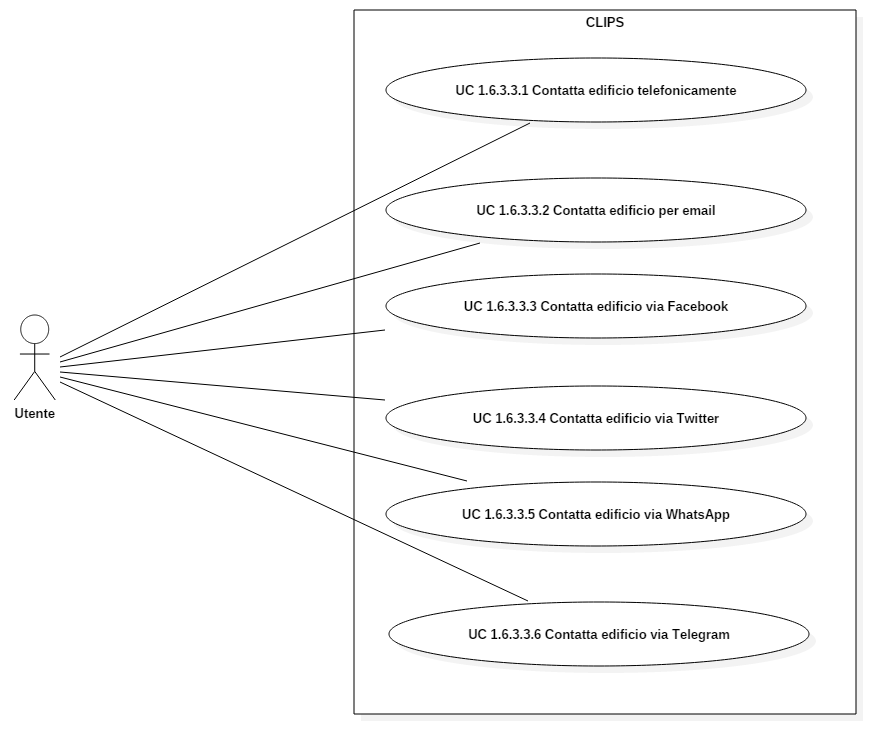
\includegraphics[scale=0.3]{img/UC_1_6_3_3.png} 
\caption{Caso d'uso UC 1.6.3.3} 
 \end{figure} 
\desc{l'utente desidera contattare l'edificio abilitato e gli viene offerta la possibilità di farlo: non è detto che tutti gli edifici mettano a disposizione tutti i canali , ma almeno uno deve essere disponibile}\\\\ 
\pre{l'utente desidera contattare un edificio}\\\\ 
\post{l'app fornisce all'utente uno o più canali attraverso cui è possibile farlo}\\\\ 
\scen{almeno uno tra i seguenti dev'essere disponibile:
 - \UC{UC1.6.3.3.1} telefonicamente,
 - \UC{UC1.6.3.3.2} per email,
 - \UC{UC1.6.3.3.3} via Facebook,
 - \UC{UC1.6.3.3.4} via Twitter,
i seguenti sono opzionali:
 - \UC{UC1.6.3.3.5} via Telegram,
 - \UC{UC1.6.3.3.6} via WhatsApp.}\\\\ 
\att{Utente}

\casoduso{UC1.6.3.3.1}{Contatta edificio telefonicamente} 
\desc{l'utente può contattare l'edificio telefonicamente}\\\\ 
\pre{l'edificio può essere contattato telefonicamente}\\\\ 
\post{il dispositivo lancia una chiamata}\\\\ 
\att{Utente}

\casoduso{UC1.6.3.3.2}{Contatta edificio per email} 
\desc{l'utente può contattare l'edificio tramite email}\\\\ 
\pre{l'edificio può essere contattato per email}\\\\ 
\post{il dispositivo lancia il client di default per la composizione di email e crea un nuovo messaggio destinato all'edificio}\\\\ 
\att{Utente}

\casoduso{UC1.6.3.3.3}{Contatta edificio via Facebook} 
\desc{l'utente può contattare l'edificio tramite Facebook}\\\\ 
\pre{l'edificio può essere contattato tramite Facebook}\\\\ 
\post{il dispositivo lancia l'applicazione di default per inviare messaggi tramite Facebook}\\\\ 
\att{Utente}

\casoduso{UC1.6.3.3.4}{Contatta edificio via Twitter} 
\desc{l'utente può contattare l'edificio tramite Twitter}\\\\ 
\pre{l'edificio può essere contattato tramite Twitter}\\\\ 
\post{il dispositivo lancia l'applicazione di default per inviare messaggi tramite Twitter}\\\\ 
\att{Utente}

\casoduso{UC1.6.3.3.5}{Contatta edificio via Telegram} 
\desc{l'utente può contattare l'edificio tramite Telegram}\\\\ 
\pre{l'edificio può essere contattato tramite Telegram}\\\\ 
\post{il dispositivo lancia Telegram aprendo una nuova conversazione con l'account fornito dall'edificio}\\\\ 
\att{Utente}

\casoduso{UC1.6.3.3.6}{Contatta edificio via WhatsApp} 
\desc{l'utente può contattare l'edificio tramite WhatsApp}\\\\ 
\pre{l'edificio può essere contattato tramite WhatsApp}\\\\ 
\post{il dispositivo lancia WhatsApp aprendo una nuova conversazione con l'account fornito dall'edificio}\\\\ 
\att{Utente}

\casoduso{UC1.7}{Modifica credenziali di accesso} 
\begin{figure}[H] 
\centering 
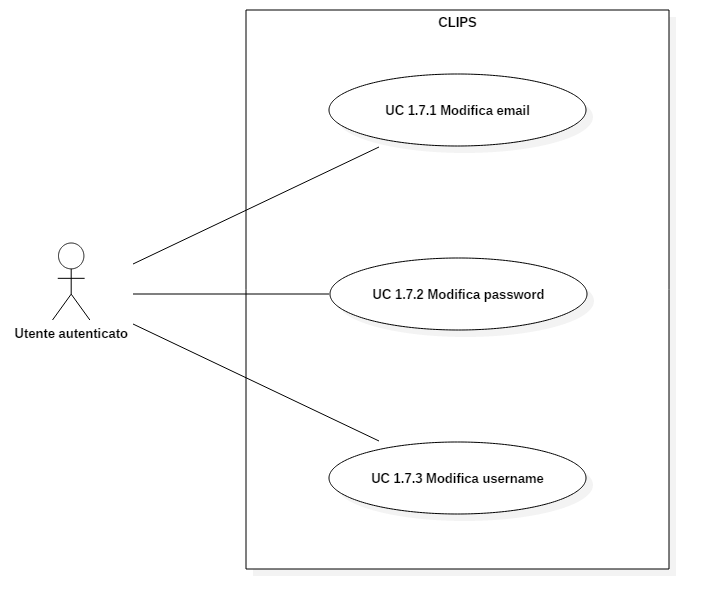
\includegraphics[scale=0.5]{img/UC_1_7.png} 
\caption{Caso d'uso UC 1.7} 
 \end{figure} 
\desc{l'utente autenticato può modificare le informazioni del login}\\\\ 
\pre{l'utente è autenticato e desidera modificare qualche informazione}\\\\ 
\post{l'informazioni che volevano essere modificate vengono modificate nel database}\\\\ 
\scen{l'utente autenticato può modificare uno dei seguenti campi:
 - \UC{UC1.7.1} l'utente autenticato modifica la mail con cui è registrato nel sito
 - \UC{UC1.7.2} l'utente autenticato modifica la password con cui esegue il login
 - \UC{UC1.7.3} l'utente modifica il proprio username}\\\\ 
\att{Utente autenticato}

\casoduso{UC1.7.1}{Modifica email} 
\desc{l'utente autenticato modifica l'indirizzo email con cui si è registrato e con cui è correntemente autenticato

ESTENSIONE:
se l'utente inserisce una password non valida il sistema restituisce un avviso e attiva \UC{UC1.1.4}}\\\\ 
\pre{l'utente è autenticato e desidera modificare l'email con cui si è registrato}\\\\ 
\post{l'utente ha modificato l'email di registrazione al sito}\\\\ 
\att{Utente autenticato}

\casoduso{UC1.7.2}{Modifica password} 
\desc{l'utente autenticato desidera modificare la password di registrazione al sistema

ESTENSIONE:
se l'utente inserisce una password che non rispetta i requisiti \Req{R0F1.2.5.4}, all'utente non viene consentito di procedere e si procede invece con \UC{UC1.1.4}}\\\\ 
\pre{l'utente è autenticato, l'utente desidera modificare la password}\\\\ 
\post{l'utente modifica con successo la password di accesso}\\\\ 
\att{Utente autenticato}

\casoduso{UC1.7.3}{Modifica username} 
\desc{l'utente autenticato desidera modificare l'username con cui compare nelle classifiche

ESTENSIONE
se l'utente inserisce un username non valido (già assegnato ad un altro utente) viene mostrata una schermata d'errore \UC{UC1.1.4}}\\\\ 
\pre{l'utente è autenticato, l'utente desidera modificare l'username}\\\\ 
\post{l'username dell'utente viene modificato}\\\\ 
\scen{l'utente è autenticato, l'utente desidera modificare l'username}\\\\ 
\att{Utente autenticato}

